\section{Einleitung}
\label{section:Einleitung}

Die Programmiersprache Ruby ist nicht für ihre Concurrency Features bekannt. In webbasierten Applikationen ist dieses Thema wichtiger den je. Die Themen Event Loop, Asynchronous vs. Synchronous und Blocking vs. Non-Blocking sind Stichwörter welche sich in vielen web-relevanten Artikeln und Blog Posts finden. Wenige dieser Artikel befassen sich jedoch mit den Grundlagen und Hintergründen dieser Begriffe. 

Mit der Bewegung Applikationen vom Desktop in die Cloud zu bringen müssen sich immer mehr Entwickler von Backend Applikatione über Performance und Skallierbarkeit ihrer Applikation gedanken machen. BenutzerInnen von Web-Applikationen erwarten sich geringste Latenzen selbst bei der Ausführung von komplexen Berechnungen auf dem Server. I/O lastige Operationen welche viele Dateien lesen und schreiben müssen, verschwenden wertvolle Server Ressourcen wenn das Lesen und Schreiben sequentiell vorgenommen wird. In vielen Fällen wird  die Performance für den EndbenutzerIn verringert

\subsection{Concurrency}
\label{section:concurrency}

Concurrency laut Robert Pike ist das behandeln von mehreren Operationen zur selben Zeit. Wenn zwei oder mehrere Prozeduren gleichzeitig behandelt werden, bedeutet das nicht zwangsweise, dass diese parallel ausgeführt werden. Jedoch besitzen Applikationen welche mehrere Operationen gleichzeitig behandeln ein nicht linearen Programmierfluss \cite[]{Pik2013}.

Werden zwei Prozeduren gleichzeitig behandelt so gibt es mehrere Möglichkeiten wie diese auf der CPU ausgeführt werden \cite[p. 14]{Erb2012}:

\begin{itemize}
  \item Sie werden sequenziell abgearbeitet (die Reihenfolge spielt dabei keine Rolle)
  \item Sie werden abwechseln abgearbeitet
  \item Sie werden parallel abgearbeitet
\end{itemize}

Alle drei Punkte können als Concurrency bezeichnet werden. Jedoch ist Punkt drei eine besondere Form von Concurrency, welcher sich Parallelismus nennt. 

\subsection{Parallelismus}

Parallelismus ist eine eine spezielle Form von Concurrency bei der zwei oder mehrere Prozeduren parallel und  zur exakt selben Zeit auf mehreren Prozessorkernen ausgeführt werden. Im Allgemeinen handelt es sich bei Parallelismus um die Art und Weise wie ein Program ausgeführt wird. In anderen Worten besitzt eine Applikation eine parallele Komponente, wenn zwei Prozeduren einer Applikation zur exakt selben Zeit einen fortschritt machen \cite[]{oracle:multithreading}.

\subsection{Concurrency vs. Parallelismus}

In der Literatur finden sich unterschiedliche Definitionen über Parallelismus und Concurrency. Oft wird zwischen diesen beiden Definitionen jedoch nicht unterschieden. 

Rob Pike ein Software Entwickler von GoLang \footnote{Konferenz Talk von Rob Pike: \url{https://vimeo.com/49718712}} versteht unter dem Begriff Concurrency das behandeln von vielen Dingen zu einem Zeitpunkt. Unter dem Begriff Parallelismus versteht er wenn zwei Prozeduren zur exakt selben Zeit auf der CPU ausgeführt werden \cite[]{Pik2013}.

Prozeduren können in folgenden Umgebungen ausgeführt werden \cite[p. 14]{Erb2012}:

\begin{itemize}
  \item Single Core Prozessoren
  \item Multi Core Prozessoren
  \item Multi Prozessoren
  \item Unterschiedliche Maschinen in einem Distributed System
\end{itemize} 

Da ein Single Core Prozessor nur eine Operation zu einem Zeitpunkt ausführen kann, ist es nicht möglich parallelität darauf zu erreichen. Auf den allen anderen genannten Umgebungen ist parallelität möglich. 

In dieser Thesis wird von Concurrency gesprochen, wenn mehrere Operationen zur selben Zeit behandelt werden.  Von Parallelität wird gesprochen, wenn zwei Prozeduren zum exact selben Zeitpunkt einen Fortschritt machen. Virtueller Parallelismus bei dem Threads durch Time-Slicing abwechselnd ausgeführt werden, wird in dieser Thesis nicht als Parallelismus bezeichnet.

\subsection{Performance}

In der Literatur findet sich keine klare Definition von Performance. Man kann sagen, dass eine Applikation performant ist, wenn diese eine Aufgabe für einen EndbenutzerIn ausführt, ohne dass die Applikation eine unangemessene Wartezeit hervorruft. Daraus kann man schließen, dass Performance im Auge des Betrachters liegt. Neben dieser wagen Definition von Performance gibt es einzelne Kategorien an denen man die Performance von zwei Applikationen vergleichen kann\cite[p. 2]{Mol2009}. 

\subsubsection{Service orientierte Performance}

\emph{Service orientierte Performance} beschreibt wie gut eine Applikation eine Aufgabe für den EndbenutzerIn zur Verfügung stellt \cite[p. 2]{Mol2009}:

\begin{itemize}
  \item {Verfügbarkeit:} beschreibt die Menge an Zeit in welcher eine Applikation für den EndbenutzerIn verfügbar ist.
  \item \emph{Antwortzeit:} beschreibt die Zeit die eine Applikation benötigt um eine Anfrage zu beantworten.
\end{itemize}


\subsubsection{Effektiv orientierte Performance}

\emph{Effektiv orientierte Performance} beschreibt wie gut eine Applikation die Ausführumgebung verwendet \cite[p. 2]{Mol2009}:

\begin{itemize}
  \item \emph{Durchsatz:} Wie viele Anfragen eine Applikation in einer Zeiteinheit verarbeiten kann.
  \item \emph{Ressourcenverbauch:} Wie viel Prozent der verfügbaren Ressourcen eine Applikation verwendet.
\end{itemize}

Das gleichzeitige Behandeln von mehreren Operationen kann zu einer gesteigerten Performance führen. Dabei können mehrere Prozeduren zur selben Zeit behandelt werden was zu einer besseren Verteilung des Ressourcenverbrauchs führen kann. Durch die Verbesserung der \emph{effekt orientierten Performance} kann die Antwortzeit für den/die EndbenuterIn verringert werden.

\subsection{I/O Operations}
\label{subsection: io_operationen}

Eine Aufgabe eines Betriebssystems ist die Verwaltung von Ein- und Ausgabe (I/O = Input/Output). I/O Operationen bezeichnet die Kommunikation zwischen der Hardware und dem Betriebssystem. Das Lesen einer Datei von einer Festplatte ist eine typische I/O Operation, welche vom Betriebssystem verwaltet wird. Eine Applikation welche eine Datei von der Festplatte lesen möchte kann einen \emph{read} Aufruf tätigen, welcher dem Betriebssystem mitteilt, dass es eine Datei lesen möchte \cite[p. 292]{tan09}.

Da I/O Operationen im Vergleich zur CPU relativ langsam sind führen diese zu längeren Antwortzeiten bei Berechnungen.  In der Zeit in der die Datei eingelesen wird  steht die gesamte Applikation still und kann keine weiteren Aufgaben ausführen. Müssen für eine Applikation viele Dateien von einer Festplatte oder über das Netzwerk eingelesen werden, kann dies zu einer erheblichen Verzögerung der Antwortzeit einer Applikation führen \cite[p. 307]{tan09}. 

Um dies zu verdeutdlichen gibt die nachfolgende Tabelle eine Übersicht über die benötigte Zeit einzelner I/O Operationen. In Spalte 3 wird die Zeit einer I/O Operation mit 1 Milliarde multipliziert um einen Vergleich mit alltäglichen Dingen des Lebens zu geben. Diese Tabelle beruht auf keinen wissenschaftlichen Quellen und sollte lediglich als grobe Referenz für die Dauer von I/O Operationen dienen. Die Tabelle beruht auf den Zahlen von Peter Norvig \cite[]{Nor98} einem Director of Research bei Google und den Vergleichen des Github Benutzers hellerbarde \cite[]{Gis15}:


\begin{figure}[!htb]
  \centering
  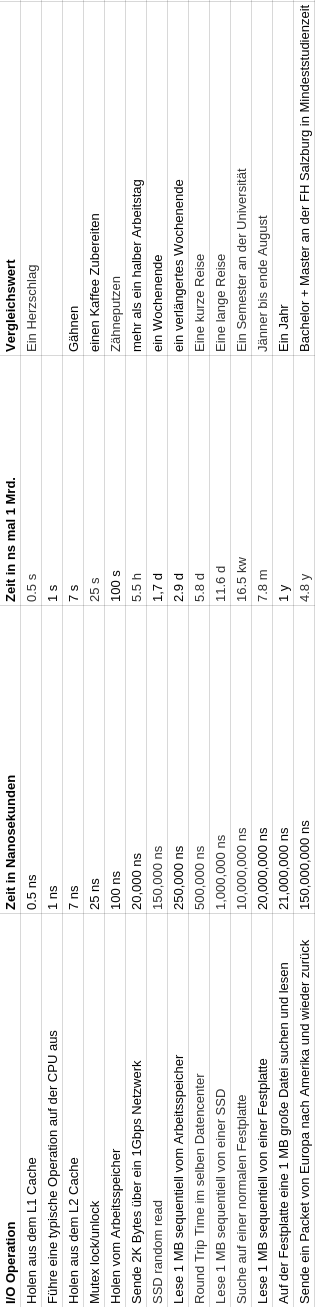
\includegraphics[width=5.5cm]{images/io_operations.png}
  \caption{
    I/O Operationen
  }
  \label{figure:syncron_vs_async}
\end{figure}